% Portable section for the revised paper. Requires amsmath, amssymb, hyperref.
% Inspected source snapshot: complextrees.com/4D/, accessed 18 September 2026.
\section{From symbolic contact to a navigable atlas}
\label{sec:explorer-methods}

The companion \emph{Connectedness Atlas} implements a common passage from a
parameter to its maps, symbolic cylinders, contact data and planar geometry.
The parameter inspector and exported specimen records retain the four coordinates
$(\alpha,\gamma,\rho,w)$ and the orientation pair. Thus a point chosen in a
three-dimensional display can be returned to an explicit planar system. The
implementation and mathematical conventions are available at
\url{https://complextrees.com/4D/}; the source snapshot discussed here was
inspected on 18 September 2026.

\subsection{Paired words and their enclosures}
Use $\lambda_-=a$, $\lambda_+=b$ and the signs $\kappa_j$ of Section~\ref{sec:core-normalization}. An accumulated cylinder map is stored as
\[
F_u(z)=t_u+L_u J_{\kappa_u}z.
\]
Appending a letter $j$ on the right gives the recurrence
\begin{equation}\label{eq:atlas-prefix-recurrence}
 t_{uj}=t_u+L_u J_{\kappa_u}(t_j),\qquad
 L_{uj}=L_u J_{\kappa_u}(\lambda_j),\qquad
 \kappa_{uj}=\kappa_u\kappa_j,
\end{equation}
where signs are multiplied. The implementation stores them as parity bits. This outermost-first convention makes
the first address symbol identify an actual first-level piece, including for
orientation-reversing maps.

The marked difference for the normalized system is
\[
D_p=\lambda_- J_{\kappa_-}(K_p)-\lambda_+ J_{\kappa_+}(K_p),
\qquad K_p\text{ is connected}\ \Longleftrightarrow\ 2\in D_p.
\]
An unequal-multiplier or reversing system is evaluated through two accumulated
maps and two parity bits. On the common direct-multiplier slice this reduces to
the usual homogeneous difference construction. Equal contraction ratios alone
do not make that reduction valid.

Let $q=\max(|\lambda_-|,|\lambda_+|)<1$ and $R=(1-q)^{-1}$.
The invariant disk $\overline B(0,R)$ supplies each word with the enclosure
\[
F_u(K_p)\subseteq \overline B(t_u,R|L_u|).
\]
A cross-prefix pair $(u,v)$ can therefore be discarded when
$|t_u-t_v|>R(|L_u|+|L_v|)$. The implementation develops the remaining pairs
in four children. Complete exhaustion gives finite separation; otherwise the
output retains a surviving frontier or the reason that a work limit stopped
the search. The browser uses this procedure to locate parameters worth refining.
For exact rational coefficients, a separate implementation replaces modulus
estimates by rational outward bounds and compares squared distances exactly.

The resulting proof object is a finite prefix antichain covering every infinite
cross-prefix address pair. Its independent checker reconstructs word maps with
rational real $2\times2$ matrices, verifies cover completeness and checks every
strict separation inequality. A successful record also supplies a positive
contact gap and an explicit product of complex parameter disks on which that
gap remains positive. This provides a constructive route from an atlas sample
to an open disconnected region in four real dimensions. It does not require
the visualization to decide membership.

\subsection{Radial surveys and three-dimensional navigation}
At a fixed weight and orientation, the survey samples the angular variables and
searches the radial interval
\[
 2\sqrt{w^2+(1-w)^2}\leq\rho\leq2.
\]
The inner endpoint comes from the closed square-sum connectedness criterion;
the outer endpoint comes from the sum-of-ratios obstruction. The current
three-orientation explorer samples an entire radial interval, brackets each
detected survival--exclusion or exclusion--survival transition, and refines
those brackets. It records re-entry bands and unresolved searches. The visible
surface uses the outermost detected finite-survival sheet. A narrow band may
fall between samples, so the recorded transition list remains part of the data.

The detailed direct--direct laboratory at \url{https://complextrees.com/4D/lab/}
contains $13\times41\times81=43\,173$ sampled rays: thirteen weights from
$0.35$ to $0.65$, with $41$ values of $\alpha$ and $81$ values of $\gamma$.
It retains two search depths, the first and outer exits, band counts and
cross-depth discrepancies. A rectangular chart displays the original stored
samples, while angular cosine interpolation and a cubic spline in weight
supply the smooth three-dimensional display. Selecting or exporting a stored
cell retains its original data. The display mesh and the radial survey therefore
have separate resolutions.

Paired letters are encoded by four symbols. The atlas can colour a parameter by
a selected surviving finite word pair or compare complete retained prefix data.
Such fields organize numerical experiments and expose changes that can be
examined through the address-equivalence relation. A constant finite label is
not used as the definition of stability. Likewise, a toroidal embedding is a
coordinate display; its imposed central hole does not classify the topology of
the connectedness locus.

\subsection{Exact families as navigable subsets}
The family registry places exact parameterized systems in the same coordinates
as the free atlas. In particular, it implements the twelve marked binary
zipper presentations obtained from three unordered planar orientation types
and four traversal signatures. Each uses the strict lens
$|z|<1$, $|1-z|<1$, evaluates its endpoint maps, and normalizes the resulting
pair. The traversal bits and the planar parity remain separate fields.
These are twelve marked presentations; no assertion that their images are
pairwise disjoint or that they classify every connected binary attractor is
needed. The comparative figures select DD$(1,0)$, DD$(1,1)$, DO$(1,0)$
and DO$(1,1)$. Their coefficient-phase projection is defined in
Section~\ref{sec:exterior-zipper-atlas}; it preserves the canonical
normalization of the registry, including the phase rotation of the
opposite map. It is a separate figure construction from the earlier
$(\alpha,\gamma)$ display of the six-specimen survey below.

The same normalization accepts the binary complex-tree families defined by
explicit eventually periodic address relations. Their records carry the raw
tree maps, the contact words, the cleared relation and the resulting normalized
parameter. The reader can therefore move between the original tree alphabet,
an algebraic contact family, a marked zipper when available, and the ambient
four-dimensional chart without changing conventions silently.

\subsection{Finite geometry, hulls and empirical difference images}
The planar renderer enumerates all words at the reported depth and carries their
first-level piece and parity. It computes in binary64 and draws binary32 vertex
buffers using a worker and WebGL~2, with a Canvas fallback. Geometry budgets
choose the actual depth; the export records that depth and the number of
prefixes drawn. Camera movement and a finer raster do not change the underlying
word set.

In exact arithmetic, with $Z_N=\{F_u(0):|u|=N\}$,
\begin{equation}\label{eq:atlas-finite-geometry-error}
 d_H(K_p,Z_N)\leq Rq^N,
 \qquad
 d_H(D_p,D_{p,N}^{\rm ctr})\leq
 (|\lambda_-|+|\lambda_+|)Rq^N,
\end{equation}
where $D_{p,N}^{\rm ctr}$ uses the two transformed copies of $Z_N$. Convexification is
nonexpansive for Hausdorff distance, so these bounds also compare the filled
finite convex hulls with the corresponding limiting convex hulls. The drawn
outlines are computed from finite floating-point centres; the analytic tail
bound does not by itself enclose every floating-point error.

The six-sample study at \url{https://complextrees.com/4D/atlas/} uses
$N=22$, hence $2^{22}$ addressed centres per attractor. Its difference images
retain word multiplicities by taking a histogram cross-correlation of the two
transformed word clouds. This represents $2^{44}$ ordered pairs without
enumerating every pair explicitly. The quantity displayed is the probability
per unit area for independent uniform finite words on the specified lattice.
A shared logarithmic opacity scale permits comparison across specimens.
For nearest-lattice rounding with spacing $h$, rounding the two clouds before
subtraction adds at most $\sqrt2 h$ of geometric displacement, in addition to
the finite-tail and arithmetic errors. This finite distribution is not assumed
to be a density of a limiting measure.


\subsection{Six linked parameter specimens}
Figures~\ref{fig:atlas-overview} and~\ref{fig:atlas-specimens} provide a linked
view of the parameter atlas and the planar sets it describes. The six samples
share $w=1/2$ and direct orientations, but generally have different complex
multipliers. Table~\ref{tab:six-specimens} records the phase representatives
and radial values used by the figures. In this display the angular embedding is
\[
 (\alpha,\gamma,\rho)\longmapsto
 \bigl((4+\rho\cos\alpha)\cos\gamma,
       \rho\sin\alpha,(4+\rho\cos\alpha)\sin\gamma\bigr).
\]
It is a visualization of a phase-chart representative, with the seam metadata
retained; it is not asserted to be a globally injective embedding of the
phase-lattice quotient. A specimen links that display position to two planar
objects: $K_p$, with its first-level decomposition, and $D_p$, with the target
point $2$. In this way the same parameter can be examined through ambient
position, geometry and finite symbolic contact information.

\begin{figure}[tbp]
\centering
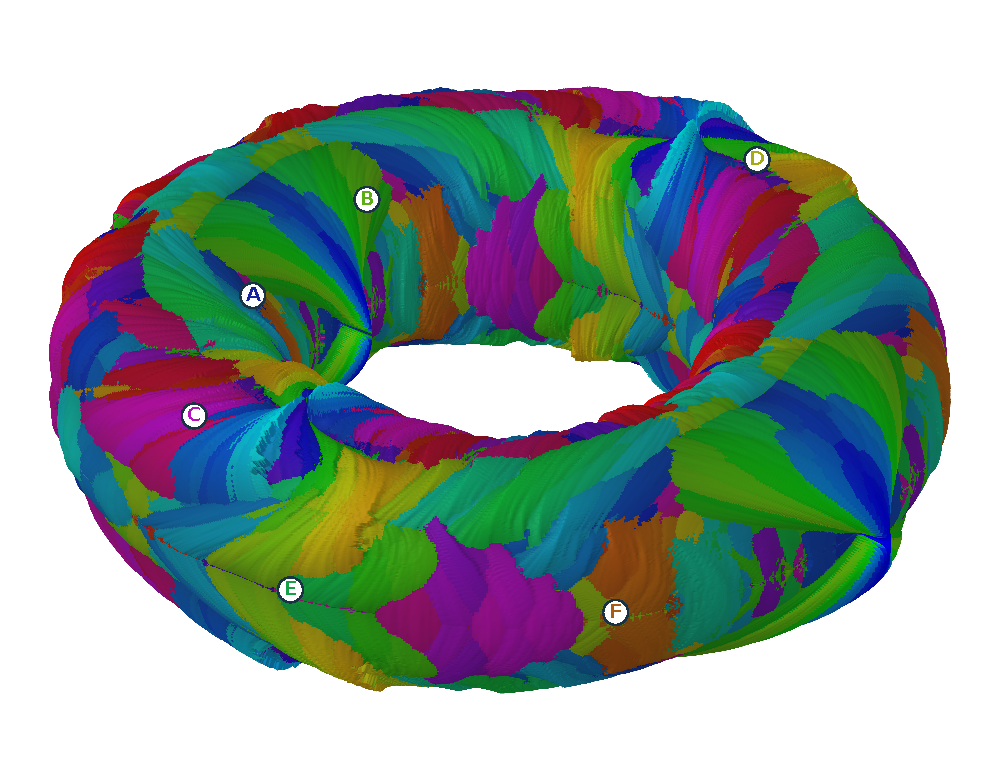
\includegraphics[width=\linewidth]{figures/Atlas_4D_Paper_Atlas.pdf}
\caption{Equal-contraction DD parameter atlas with specimens A--F. The angular
view displays the finite numerical study underlying the companion explorer.
Colours record selected finite pair-address codes. The central hole belongs
to the coordinate display. Parameters are given in
Table~\ref{tab:six-specimens}, with planar sets in
Figure~\ref{fig:atlas-specimens}.}
\label{fig:atlas-overview}
\end{figure}

\begin{figure}[tbp]
\centering
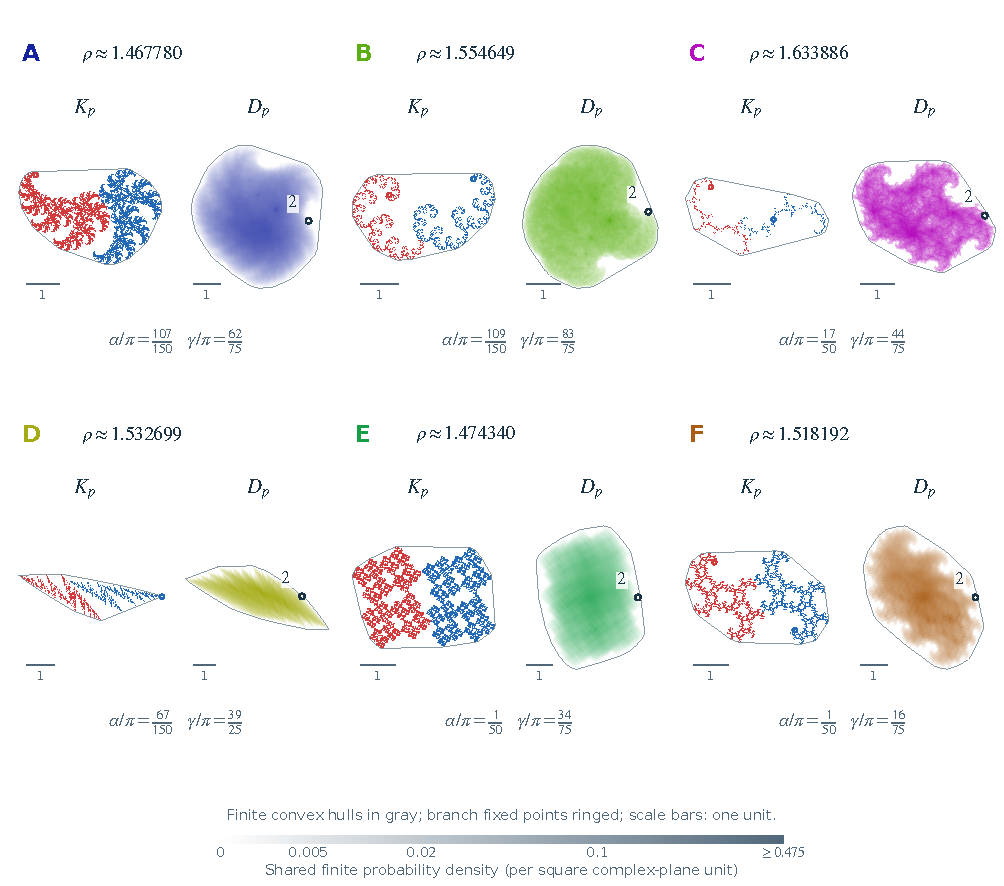
\includegraphics[width=\linewidth]{figures/Atlas_4D_Paper_Specimens.pdf}
\caption{The six linked specimens. Red and blue show first-level pieces of
$K_p$; $D_p=aK_p-bK_p$ uses the corresponding atlas hue and a shared finite
probability-density scale. Every attractor uses all length-22 addressed
centres. Gray outlines are finite convex hulls, rings in $K_p$ mark branch
fixed points, and the ring in $D_p$ marks $2$. Scale bars have length one;
panels are fitted independently. The images do not certify exact contact.}
\label{fig:atlas-specimens}
\end{figure}
\begin{table}[tbp]
\centering\small
\begin{tabular}{@{}crrrrr@{}}
\toprule
Sample & $\alpha/\pi$ & $\gamma/\pi$ & $\rho$ & $Rq^{22}$ & $2qRq^{22}$\\
\midrule
A & $\frac{107}{150}$ & $\frac{62}{75}$ & 1.4677798748 & $6.76\mathbin{\times}10^{-4}$ & $9.21\mathbin{\times}10^{-4}$ \\
B & $\frac{109}{150}$ & $\frac{83}{75}$ & 1.5546487570 & $1.70\mathbin{\times}10^{-4}$ & $2.19\mathbin{\times}10^{-4}$ \\
C & $\frac{17}{50}$ & $\frac{44}{75}$ & 1.6338859797 & $5.25\mathbin{\times}10^{-5}$ & $6.43\mathbin{\times}10^{-5}$ \\
D & $\frac{67}{150}$ & $\frac{39}{25}$ & 1.5326993465 & $2.39\mathbin{\times}10^{-4}$ & $3.12\mathbin{\times}10^{-4}$ \\
E & $\frac{1}{50}$ & $\frac{34}{75}$ & 1.4743398428 & $6.07\mathbin{\times}10^{-4}$ & $8.24\mathbin{\times}10^{-4}$ \\
F & $\frac{1}{50}$ & $\frac{16}{75}$ & 1.5181920528 & $3.00\mathbin{\times}10^{-4}$ & $3.96\mathbin{\times}10^{-4}$ \\
\bottomrule
\end{tabular}
\caption{Parameters of the six equal-contraction DD specimens ($w=1/2$),
with $q=1/\rho$. Radial values are rounded here; the full numerical record
is retained in the source. The last columns are analytic tail estimates
in exact arithmetic, excluding floating-point and density-grid errors.}
\label{tab:six-specimens}
\end{table}

\subsection{Reproducible states and figures}
The mathematical record consists of coefficients, orientations, word convention,
sampled grids, budgets, retained evidence and arithmetic. The figure record adds
the camera, projection, raster, display mesh, colour map and finite geometric
depth. The explorer exports these independently of the image through JSON
records and embeds parameter metadata in PNG files. The detailed laboratory
also provides raw slice CSV and validated session records. These records allow a
figure to be reproduced while preserving the distinction between a mathematical
parameter, the computation performed there and its visual presentation.
